\documentclass[landscape,fontscale=1,margin=0.2cm,paperwidth=70truecm, paperheight=40truecm,debug]{baposter}
\usepackage{multirow}
\begin{document}

\begin{poster}{
  headerheight=60pt,
  columns=5,
  background=plain,
%   linewidth=0.5pt,
  borderColor=orange!70,
  textborder=rectangle,
  headershade=plain,
  headerColorOne=orange!80,
  headershape=smallrounded,
  boxheaderheight=1.5em,
  headerfont={},
  boxColorOne=white,
  bgColorOne=darkgray,
  bgColorTwo=blue!60,
}{}{\Large{\color{white}{U.S. Coast Guard Information Technician Cheat Sheet}}}{}{d}

%%%%%%%%%%%%%%%%%%%%%%%%%%%%%%%%%%%%%%%%%%%%%%%%%%%%%%%%%%%%%%%%%%%%%%%%%%%%%%
\begin{posterbox}[column=0]{Traffic Analysis Terms}
\begin{description}
\item[Traffic Load] the ratio of call arrivals in a specified period of time to the average amount of time taken to service each call during that period.
\item[erlang](E) One erlang is 3600 seconds of calls on the same circuit, or enough traffic load to keep one circuit busy for 1 hour.  
\item[Centum Call Seconds] One CCS is 100 seconds of calls on the same circuit.
\item[Average Hold Time] AHT is the total time of all calls in a specified period divided by the number of calls in that period.
\item[Busy Hour Traffic] the hour of the day with the highest traffic intensity is called the busy hour. In this case, the daily peak traffic intensity is also called busy hour traffic or busy hour usage. Busy hour traffic is the number of erlangs or CCS used during the busy hour.
\item[Peg count] is the number of calls in a specified period of time.
\item[Busy peg] the number of times a trunk group is accessed to make an outgoing call and it is in use or busy.
\item[Grade of Service] (GoS) is defined as the probability that calls will be blocked while attempting to seize circuits.
\item[Carried traffic] is the traffic that is actually serviced by telecommunications equipment.
\item[Offered traffic] is the actual amount of traffic attempts on a system.
\item[Daily Peak Period] (DPP) records the highest traffic volume measured during a day. This method requires continuous measurement and is typically used in environments where the peak hour may be different from day to day.
\item[Fixed Daily Measurement Interval](FDMI) requires measurements only during the predetermined peak periods. It is used when traffic patterns are somewhat predictable and peak periods occur at regular intervals. Business traffic usually peaks around 10:00 a.m. to 11:00 a.m. and 2:00 p.m. to 3:00 p.m.

\end{description}
\end{posterbox}

\begin{posterbox}[column=0,below=auto,textborder=rounded]{Queueing Theories}
\textbf{Blocked Calls} A blocked call is a call that is not serviced immediately. Calls are considered blocked if they are rerouted to another trunk group, placed in a queue, or played back a tone or announcement. The nature of the blocked call determines the model you select because blocked calls result in differences in the traffic load. Here are the main type of blocked calls:
\begin{description}
\item[Blocked Calls Held] These blocked calls are lost, never to come back again. 
\item[Blocked Calls Cleared] These blocked calls are cleared from the system, meaning that when a caller is blocked, the call goes somewhere else (mainly to other traffic-sensitive facilities).
\item[Blocked Calls Delayed] These blocked calls remain on the system until facilities are available to service the call.
\item[Blocked Calls Retried] BCR assumes that once a call is blocked, a percentage of the blocked callers retry and all other blocked callers retry until they are serviced. BCR is a derivative of the BCC model and is used in the Extended Erlang B model.
\end{description}
\begin{center}
\begin{tabular}{lll}
Erlang B & Blocked Calls Cleared & Users must redial until connected\\
Erlang C & Blocked Calls Delayed & Call overflows to another Trunk\\
Poisson & Blocked Calls Held & Call is placed in a holding circuit\\
\end{tabular}
\begin{tabular}{lll}
Erlang B & BCC & Erlang B $\rightarrow$ C \\
Erlang C & BCD & Erlang C $\rightarrow$ D \\
Poisson & BCH & Poisson $\rightarrow$ PH\\
\end{tabular}

\end{center}
\end{posterbox}

\begin{posterbox}[column=0,below=auto,height=bottom]{Traffic Load Measurements}
\begin{center}
\begin{tabular}{|c|c|}
\hline
Traffic Load Measurement & Example\\\hline

AHT = $\frac{total~call~seconds}{calls}$ & 172.87 = $\frac{3976}{23}$\\
&\\
erlangs = $\frac{calls~*~AHT}{one~erlang}$ & 1.104 = $\frac{23 * 172.87}{3600}$\\
&\\
CCS = $\frac{calls~*~AHT}{100}$ & 39.76 = $\frac{23 * 172.87}{100}$\\\hline
\end{tabular}
\end{center}
\begin{itemize}
\item erlang = 36 CCS = 3600 seconds of calls on the same circuit.
\item CCS = 100 seconds of calls on the same circuit.
\end{itemize}
\begin{center}
\begin{tabular}{|c|c|}
\hline
CCS to erlang&erlang to CCS\\\hline
CCS = $erlangs~ *~36$ & erlangs = $\frac{CCS}{36}$\\\hline
\end{tabular}
\end{center}
\end{posterbox}
\begin{posterbox}[column=1]{Erlang B}
\[
B(c,a) = \frac{\frac{a^c}{c!}}{\sum\limits_{k=0}^{c} \frac{a^k}{k!}}
\]
\begin{itemize}
\item B(c,a) probability of blocking a call
\item c is the number of circuits
\item a is the traffic load
\end{itemize}
\[
B(8,4.53) = \frac{\frac{4.53^8}{8!}}{\sum\limits_{k=0}^{8}\frac{4.53^k}{k!}}
\]
\[
B(8,4.53) = \frac{4.39809992845264833770089\overline{285714}}{\sum\limits_{k=0}^{8}\frac{4.53^k}{k!}}
\]
\[
B(8,4.53) = \frac{4.39809992845264833770089\overline{285714}}{\sum\limits_{k=0}^{8} (1 + 4.53 + 10.26045 +}
\]
\[
15.4932795 + 17.54613903375 + 15.8968019645775 +
\]
\[
 12.0020854832560125 + 7.767063891307105232\overline{142857})
\]
\[
\]
\[
B(8,4.53) = \frac{4.39809992845264833770089\overline{285714}}{84.495819872890617732142857}
\]
\[
B(8,4.53) = 0.0520510947768638832211314889713364792038405723028320
\]
\[
B(8,4.53) = 5\%
\]

\end{posterbox}
\begin{posterbox}[column=1,below=auto]{Erlang C}
\[
C(c,a) = \frac{\frac{a^c~c}{c!(c-a)}}{\sum\limits_{k=0}^{c-1}\frac{a^k}{k!} + \frac{a^c~c}{c!(c-a)}}
\]
\begin{itemize}
\item C(c,a) probability of call delay
\item c is the number of circuits
\item a is the traffic load
\end{itemize}
\[
C(5,1.5) = \frac{\frac{1.5^5~5}{5!(5-1.5)}}{\sum\limits_{k=0}^{5-1}\frac{1.5^k}{k!} + \frac{1.5^5~5}{5!(5-1.5)}}
\]
\[
C(5,1.5) = \frac{0.0904017\overline{857142}}{\sum\limits_{k=0}^{5-1}\frac{1.5^k}{k!} + 0.0904017\overline{857142}}
\]
\[
C(5,1.5) = \frac{0.0904017\overline{857142}}{\frac{563}{128} + 0.0904017\overline{857142}} = 0.02013923421181619...
\]
\[
C(5,1.5) = 0.0201392...
\]

\end{posterbox}

\begin{posterbox}[column=1,below=auto,height=bottom]{Poisson}
\[
P(c,a) = 1 - e^{-a} \sum\limits_{k=0}^{c-1} \frac{a^k}{k!}
\]
\begin{itemize}
\item P(c,a) probability of blocking a call
\item $e$ is the natural log base
\item c is the number of circuits
\item a is the traffic load
\end{itemize}
\[
P(9,4.69) = 1 - e^{-4.69} \sum\limits_{k=0}^{9 - 1}\frac{4.69^k}{k!}
\]
\[
P(9,4.69) = 1 - e^{-4.69} \sum\limits_{k=0}^{9-1} = ( 1 + 4.69 + 10.99805 + 17.1936181\bar{6} + 20.15951730041\bar{6}
\]
\[
+ 18.9096272277908\bar{3} + 14.7810252830565013\bar{8} + 9.903286939647855930\bar{5} + 
\]
\[
5.80580196836855553928819\bar{4}) = 103.440926879279742849788194
\]
\[
1 - e^{-4.69}(103.440926879279742849788194) = 0.0497207...
\]
\[
P(9,4.69)= 5\% 
\]
\end{posterbox}

\begin{posterbox}[column=2]{NetOps}
\begin{description}
\item[INFOCON 5] routine network operations (NetOps); this occurs when ``baselining'' should be accomplished and maintained. Baselining is discussed with additional detail in the next section.
\item[INFOCON 4] increases NetOps readiness in preparation for operations or exercises, with limited impact to the end-user.
\item[INFOCON 3] further increases NetOps readiness by increasing the frequency of validation of the information network and its corresponding configuration. Impact to end-users is minor.
\item[INFOCON 2] further increase in frequency of validation of the information network and its corresponding configuration. Increased impact to network administrators. Can benefit from ``hot spare'' equipment which reduces downtime by allowing rebuilding in parallel. Impact to end-users could be significant for short periods, which can be mitigated through training and scheduling.
\item[INFOCON 1] highest readiness condition which addresses intrusion techniques that cannot be identified or defeated at lower readiness levels (e.g. kernel root kits) Impact on administrators is significant. Impact to end-users could be significant for short periods, which can be mitigated through training and scheduling.
\end{description}
\end{posterbox}
\begin{posterbox}[column=2,below=auto,textborder=rounded]{Grounding}
\begin{description}
\item[NEC article 250] Grounding of Power Services.
\item[NEC article 800] Grounding of Communication Circuits.
\end{description}
\end{posterbox}
\begin{posterbox}[column=2,below=auto,textborder=rounded]{RJ-45-568A}
\begin{center}
\includegraphics{RJ-45_TIA-568A_Left.png}\includegraphics[scale=0.2]{pinpair.png}
\end{center}
\textbf{Mnemonic}
Grass O Sky O Dirt A
\end{posterbox}
\begin{posterbox}[column=2,below=auto,textborder=rounded]{Color-coding of specific termination fields}
\begin{center}
\begin{tabular}{lll}
Termination Type & Color & Typlical Application\\\hline
demarcation point & \color{orange}{orange} & central office connection\\
network connection & \color{green}{green}& user side of central office connection\\
cabling subsystem 3 & \colorbox{darkgray}{\color{white}{white}}& First-level backbone\\
cabling subsystem 2 & \color{gray}{gray} & Second-level backbone\\
campus cabling & \color{brown}{brown} & termination of campus cable between buildings\\
cabling subsystem 1 & \color{blue}{blue} & termination of station telecommunications media\\
miscellaneous & \colorbox{darkgray}{\color{yellow}{yellow}} & alarms, security, or energy management
\end{tabular}
\end{center}
\end{posterbox}
\begin{posterbox}[column=2,below=auto]{OSI Model}
\begin{center}
\rowcolors{1}{orange!20}{red!05}
\begin{tabular}{|l|l|l|l|}
\hline
\multicolumn{4}{ |c| }{OSI Model}\\
\hline
\hline
& Layer Number& Layer Name & Function\\\hline
Data & 7 & Application & Network process to application\\
 & 6 & Presentation & Convert machine data\\
 & 5 & Session & Interhost communication\\\hline
Segments & 4 & Transport & End-to-End connections\\\hline
Packet/Datagram & 3 & Network & Path determination\\\hline
Frame & 2 & Data link & Physical addressing\\\hline
Bit & 1 & Physical & binary transmission\\\hline
\end{tabular}
\end{center}
\textbf{Mnemonic}\\
The Physical Data Network Must Transport the Session Presentation to the Application.
\end{posterbox}
\begin{posterbox}[column=2,below=auto]{Communication Standards}
\begin{description}
\item[Primary Rate ISDN (ISDN-PRI)] has 23 bearer channels (64 kbit/s each) for a \textbf{\color{orange}{combined data rate of 1.5 Mbit/s}} (US standard).
\item[T1 or DS1] A DS1 circuit is made up of twenty-four 8-bit channels (also known as timeslots or DS0s), each channel being a 64 kbit/s DS0 multiplexed carrier circuit. A DS1 is also a full-duplex circuit, which means the circuit transmits and receives 1.544 Mbit/s concurrently.
\item[T3 or DS3] This level of carrier \textbf{\color{orange}{can transport 28 DS1(T3) level signals}} within its payload. The data rate for this type of signal is 44.736 Mbit/s (45 Mb).
\end{description}
\end{posterbox}
\begin{posterbox}[column=3,textborder=rounded]{Uninterruptible Power Supply Types}
\begin{description}
\item[Standby] also called an ``offline UPS'' draws AC current from the outlet and switches to the battery after detecting a loss of power. This switch only takes milliseconds, and is often unnoticed.
\item[Line Interactive] interacts with the AC power to smooth out the waveforms and correct the rise and fall of voltage.
\item[Online] the most advanced UPS. The inverter rectifies incoming AC power to DC current, which charges the battery, and then changes the DC current back to AC to provide clean power. In this case, the protected equipment never receives power directly from the AC source. These units contain cooling fans, which have the potential to influence your telecommunications room's environment (i.e. sound, temperature).
\end{description}
\end{posterbox}
\begin{posterbox}[column=3,below=auto]{UPS purposes}
\begin{center}
The Coast Guard primarily uses a UPS in one of three ways:
\end{center}
\begin{description}
\item[Provide emergency power] During the total loss of commercial power, a UPS will carry the load of all equipment plugged into the UPS for an amount of time.
\item[Provide clean power] Commercial power is not always ``clean''. In some instances, the AC power in a building will not be uniform, or can be susceptible to voltage spikes or drops.
\item[Unattended shutdown] The design of orderly shutdown from the software prevents data loss or data corruption by properly terminating applications instead of just cutting off the power. 
\end{description}
\end{posterbox}
\begin{posterbox}[column=3,below=auto,textborder=rounded]{UPS: Determining System Power Requirements}
\begin{description}
\item[Amperage] multiply the number of amps by the nominal line voltage. (Nominal line voltage for North America is 120)
\item[Wattage] multiply the number of watts by 1.4.
\end{description}
\end{posterbox}
\begin{posterbox}[column=3,below=auto]{Types of Backups}
\begin{description}
\item[Full] This type backs up all selected files and directories and clears the archive attributes. This backup type is normally conducted weekly and serves as the foundation for other types of backups.
\item[Incremental] During this type of backup the software backs up only the files or directories that have changed since the last Full or Incremental backup. The software establishes which files have changed based on the status of the archive attributes. \textbf{This type of backup clears the archive attributes}.
\item[Differential] This type of backup is the same as an Incremental backup, however the software doesn't clear the archive attribute, thus all files and directories that have changed since the previous Full are backed up.
\end{description}
\end{posterbox}
\begin{posterbox}[column=3,below=auto,textborder=rounded]{Advantages of Backups}
\begin{itemize}
\item The advantage of an \textbf{\color{orange}{Incremental}} backup over a Differential is \textbf{\color{orange}{less space used}} on the backup media.
\item The advantage of a \textbf{\color{orange}{Differential}} over an Incremental is \textbf{\color{orange}{faster restoration time}}.
\end{itemize}
\end{posterbox}
\begin{posterbox}[column=3,below=auto]{Physical Security}
\begin{description}
\item[Exclusion Area] An exclusion area is the \textbf{\color{orange}{most secure}} type of restricted area. It may be located within a less secure type of restricted area. Access to the exclusion area constitutes, or is considered, actual access to the security interest or asset
\item[Limited Area] A limited area is the \textbf{\color{orange}{second most secure}} type of restricted area. It may be located inside a controlled area, but is never inside an exclusion area. Uncontrolled or unescorted movement could permit access to the security interest or asset
\item[Controlled Area] A controlled area is the \textbf{\color{orange}{least secure}} type of restricted area. It may also serve as a buffer zone for exclusion and limited areas, thus providing administrative control and protection against sabotage, disruption, or potentially threatening acts. Uncontrolled movement may or may not permit access to the security interest or asset
\end{description}
\end{posterbox}
\begin{posterbox}[column=3,below=auto,height=bottom]{Basic color codes for AC wiring}
\begin{tabular}{llll}
\includegraphics[scale=0.8]{Color_wire_black.png}& Hot 115 VAC & \includegraphics[scale=0.8]{Color_wire_white.png}&Neutral, return path from hot wire.\\
\includegraphics[scale=0.8]{Color_wire_green_yellow.png}& Ground & \includegraphics[scale=0.8]{Color_wire_red.png}& Hot, 115 VAC for 220-240 VAC.
\end{tabular}
\end{posterbox}
\begin{posterbox}[column=4]{25 pair color code}
\begin{description}
\item[Group One] white, red, black, yellow, violet.
\item[Group Two] blue, orange, green, brown, slate.
\end{description}
\begin{description}
\item[Group One Mnemonic] \colorbox{black}{\color{white}{Winchester}} \color{red}{Rifles} \color{black}{Bring} \colorbox{black}{\color{yellow}{You}} \color{purple}{Victory}
\item[Group Two Mnemonic] \color{blue}{B}\color{orange}{O}\color{green}{G}\color{brown}~{Br}u\color{gray}{Sh}
\end{description}
\begin{center}
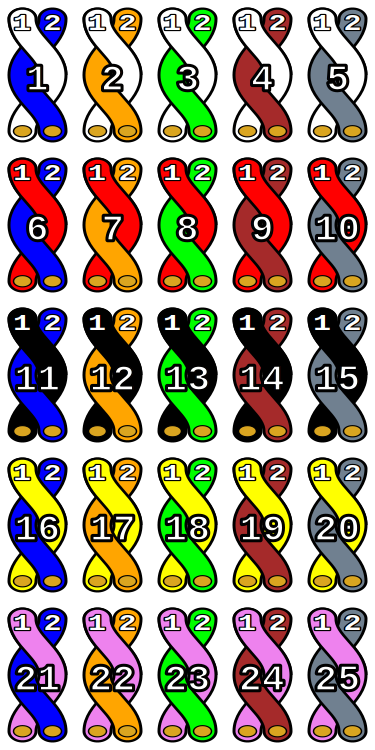
\includegraphics[scale=0.5]{25_pair_color_code_chart.png}
\end{center}
\end{posterbox}


\end{poster}

\end{document}

